\documentclass[12pt, a4paper]{article}
\usepackage{amsmath}
\usepackage[sc]{mathpazo}
\usepackage[a4paper]{geometry}
\usepackage{datetime}
\usepackage[myheadings]{fullpage}
\usepackage{fancyhdr}
\usepackage{lastpage}
\usepackage{graphicx, wrapfig, subcaption, setspace, booktabs}
\usepackage[T1]{fontenc}
\usepackage[font=small, labelfont=bf]{caption}
\usepackage{fourier}
\usepackage[protrusion=true, expansion=true]{microtype}
\usepackage[english]{babel}
\usepackage{sectsty}
\usepackage{url, lipsum}
\usepackage{hyperref,bookmark}
\usepackage[T1]{fontenc}
\usepackage{amssymb}
\usepackage{tabularx}
\usepackage{listings}
\usepackage{xcolor}
\usepackage{longtable}
\usepackage{setspace}
\usepackage{float}
\usepackage[ruled,linesnumbered]{algorithm2e}

\providecommand{\tightlist}{%
	\setlength{\itemsep}{0pt}\setlength{\parskip}{0pt}}

\usepackage{lmodern}
\usepackage{amssymb,amsmath}
\usepackage{ifxetex,ifluatex}
\usepackage{fixltx2e} % provides \textsubscript
\ifnum 0\ifxetex 1\fi\ifluatex 1\fi=0 % if pdftex
\usepackage[T1]{fontenc}
\usepackage[utf8]{inputenc}
\usepackage{textcomp} % provides euro and other symbols
\else % if luatex or xelatex
\usepackage{unicode-math}
\defaultfontfeatures{Ligatures=TeX,Scale=MatchLowercase}
\fi
% use upquote if available, for straight quotes in verbatim environments
\IfFileExists{upquote.sty}{\usepackage{upquote}}{}
% use microtype if available
\IfFileExists{microtype.sty}{%
	\usepackage[]{microtype}
	\UseMicrotypeSet[protrusion]{basicmath} % disable protrusion for tt fonts
}{}
\IfFileExists{parskip.sty}{%
	\usepackage{parskip}
}{% else
	\setlength{\parindent}{0pt}
	\setlength{\parskip}{6pt plus 2pt minus 1pt}
}
\usepackage{hyperref}
\hypersetup{
	pdfkeywords={bolt, bolts, coarse, diameter, DIN, eye, fine, grade, hex, identify,
		inch, inner, ISO, l-bolt, lifting, marking, measurement, metric, nut,
		nuts, outer, SAE, size, step, thread, u-bolt, UNC, UNF, UNJC, UNJF,
		UNRC, UNRF, UTS, wing},
	pdfborder={0 0 0},
	breaklinks=true}
\urlstyle{same}  % don't use monospace font for urls
\usepackage{longtable,booktabs}
% Fix footnotes in tables (requires footnote package)
\IfFileExists{footnote.sty}{\usepackage{footnote}\makesavenoteenv{longtable}}{}
\usepackage{graphicx,grffile}
\makeatletter
\def\maxwidth{\ifdim\Gin@nat@width>\linewidth\linewidth\else\Gin@nat@width\fi}
\def\maxheight{\ifdim\Gin@nat@height>\textheight\textheight\else\Gin@nat@height\fi}
\makeatother
% Scale images if necessary, so that they will not overflow the page
% margins by default, and it is still possible to overwrite the defaults
% using explicit options in \includegraphics[width, height, ...]{}
\setkeys{Gin}{width=\maxwidth,height=\maxheight,keepaspectratio}
\setlength{\emergencystretch}{3em}  % prevent overfull lines
\providecommand{\tightlist}{%
	\setlength{\itemsep}{0pt}\setlength{\parskip}{0pt}}
\setcounter{secnumdepth}{0}
% Redefines (sub)paragraphs to behave more like sections
\ifx\paragraph\undefined\else
\let\oldparagraph\paragraph
\renewcommand{\paragraph}[1]{\oldparagraph{#1}\mbox{}}
\fi
\ifx\subparagraph\undefined\else
\let\oldsubparagraph\subparagraph
\renewcommand{\subparagraph}[1]{\oldsubparagraph{#1}\mbox{}}
\fi

% set default figure placement to htbp
\makeatletter
\def\fps@figure{htbp}
\makeatother

\ifnum 0\ifxetex 1\fi\ifluatex 1\fi=0 % if pdftex
%\usepackage[shorthands=off,main=english]{babel}
%\else
% load polyglossia as late as possible as it *could* call bidi if RTL lang (e.g. Hebrew or Arabic)
%\usepackage{polyglossia}
%\setmainlanguage[]{english}
%\fi

\pagestyle{fancy}
\fancyhf{}
\setlength\headheight{15pt}
\fancyhead[L]{Luis Fernando Enriquez-Contreras}
\fancyhead[R]{Motor Mounting SOP}
\fancyfoot[R]{Page \thepage\ of \pageref{LastPage}}


\begin{document}
	%-------------------------------------------------------------------------------
	% Title
	%-------------------------------------------------------------------------------
	\begin{titlepage}
		
		\newcommand{\HRule}{\rule{\linewidth}{0.5mm}} % Defines a new command for the horizontal lines, change thickness here
		
		\center % Center everything on the page
		
		%---------------------------------------------------------
		%	HEADING SECTIONS
		%---------------------------------------------------------
		
		\textsc{\LARGE University of California, Riverside}\\[1.5cm] % Name of your university/college
		\textsc{\Large Bourns College of Engineering}\\[0.5cm] % Major heading such as course name
		\textsc{\large College of Engineering, Center for Environmental Research and Technology (CE-CERT) }\\[0.5cm] % Minor heading such as course title
		
		%---------------------------------------------------------
		%	TITLE SECTION
		%---------------------------------------------------------
		
		\HRule \\[0.6cm]
		{\Large Motor Mounting Standard Operating Procedure }\\[0.4cm] % Title of your document
		\HRule \\[1.0cm]
		
		%---------------------------------------------------------
		%	AUTHOR SECTION
		%---------------------------------------------------------
		
		%\begin{minipage}{0.4\textwidth}
		\begin{center} \large
			% \emph{Authors:}  
			\medskip
			{\textsc{\textbf{Luis Fernando Enriquez-Contreras} }} 
		\end{center}
		%\end{minipage}
		
		
		%---------------------------------------------------------
		%	DATE SECTION
		%---------------------------------------------------------
		\begin{center}
%			\selectlanguage{USenglish}
			{\large September 20, 2022}
		\end{center}
		% Date, change the \today to a set date if you want to be precise
		
		%---------------------------------------------------------
		%	LOGO SECTION
		%---------------------------------------------------------
		%\vfill
		\newcommand*{\plogo}{
\includegraphics{UC_Riverside_seal.pdf}}
%		\newcommand*{\plogo}{
\includegraphics[width=0.25\textwidth]{UC_Riverside_seal.pdf}}
		
		\plogo\\[1cm] % Include a department/university logo - this will require the graphicx package
		
		%---------------------------------------------------------
		
		\vfill % Fill the rest of the page with whitespace
	\end{titlepage}
	
	\newpage
	
	%-------------------------------------------------------------------------------
	% Table of Contents and Figures
	%-------------------------------------------------------------------------------
	\doublespacing
	\tableofcontents
	\pagebreak
	\listoffigures
	\listoftables
	\lstlistoflistings  
	\pagebreak
	
	%-------------------------------------------------------------------------------
	% Abstract
	%-------------------------------------------------------------------------------
	
	%-------------------------------------------------------------------------------
	% BODY
	%-------------------------------------------------------------------------------
	
	\part{Introduction}
	 	Motor Testing requires the mounting of the motor, torque transducer, and generator. This guide explains the parts needed, and how and where to order them.
	 	
	\part{Frame Manufacturer} 
		The job is to either test a motor or a generator. Usually the product is prototype, and will not have a standard mounting system. A frame will need to be created to mount the motor/generator to the testbench.
		
	\part{L-Type Jaw Coupling}
		The shafts of the motor, torque transducer, and generator are connected by L-Type Jaw Couplings. These couplings interlock with a rubber component called a spider. The coupling secures with the shaft with a hex screw. A key stock is a metal rectangular prism the locks the shaft and coupling to prevent slippage. The shafts may have different diameters, but the couplings come in different shaft sizes. For exapmple, an L-150 coupling will have the same diameter regardless if it is a 7/8" 1.5" diameter.  The jaw coupling size does not affect keyway size, for example, the 7/8 in. L-100 coupling you use and the 7/8in L-150 coupling we use have the same keyway dimensions, meaning they both use the same keystock. We have multiple couple at ce-cert, but new one may be need needed if none fit the shaft of the prototype.		
	
	\part{Fastners}
	    Bolts and nut ar need to faten on motors, please refer to this guide from: to make a descion of the correct nut and bolt.
		\hypertarget{introduction-to-nut-and-bolt-sizes}{%
			\section{\texorpdfstring{{Introduction to Nut and Bolt
						Sizes}}{Introduction to Nut and Bolt Sizes}}\label{introduction-to-nut-and-bolt-sizes}}
		
		\hypertarget{isolation-scope-ifxaekaopxrq6yt1cpor23715}{}
		
		\hypertarget{idgbn}{}
		\hypertarget{iz9k}{}
		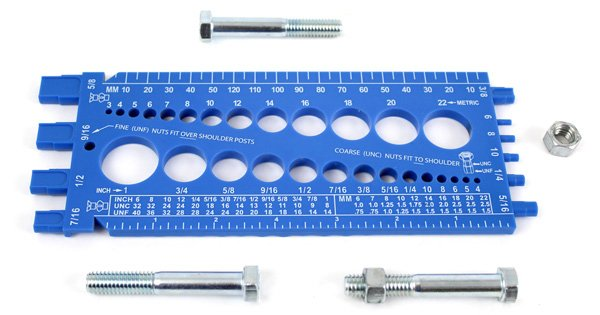
\includegraphics{Introduction to Nut and Bolt Sizes_files/62ffc530cd49d888286820.jpg}
		
		\hypertarget{ikxe}{}
		When discussing nut and bolt sizes, it is not only important to
		understand the differences between inch and metric fasteners, but to
		also understand which measurements are essential to determining the
		sizes of the nuts and bolts you need for your applications.
		
		\hypertarget{iov0gj}{}
		All sizes of nuts and bolts fall into one of two main categories:
		\emph{standard/inch} and \emph{metric} . While it may seem natural to
		look for imperial nut and bolt sizes when searching for fasteners
		measured in inches, the industry does not use this term. Instead, you
		will find \emph{standard, inch, or U.S.} fasteners. Fortunately,
		\emph{metric} is the only industry term for fasteners measured in
		millimeters.
		
		\hypertarget{ivhqvk}{%
			\subsection{Differences Between Inch and Metric Nuts and
				Bolts}\label{ivhqvk}}
		
		\hypertarget{igonwo}{}
		While the functionality and physical characteristics of inch and metric
		\href{https://www.huyett.com/all-products/nuts}{nuts} and
		\href{https://www.huyett.com/all-products/bolts}{bolts} are essentially
		the same, how they are sized is different. The sizes are communicated by
		key measurements, standards, and strength grade markings.
		
		\hypertarget{im7ycf}{}
		The biggest difference between nut and bolt inch and metric sizes is how
		measurements are defined. While each type of nut or bolt will have its
		own set of characteristics to measure, every fastener is measured by its
		\emph{thread diameter} and \emph{threads per inch (TPI)} or \emph{thread
			pitch} .
		
		\hypertarget{ik45sl}{%
			\subsubsection{Thread Measurements}\label{ik45sl}}
		
		\hypertarget{in0inq}{}
		Regardless of inch or metric measurements, thread diameter is defined by
		either the outside diameter (OD) or the inside diameter (ID) of the
		part:
		
		\hypertarget{ihbijz}{%
			\paragraph{Outside Diameter (OD) or Major Diameter}\label{ihbijz}}
		
		\begin{itemize}
			\tightlist
			\item
			\textbf{Nuts:} the distance between the roots of the threads
			\item
			\textbf{Bolts:} the distance between the crests of the threads
		\end{itemize}
		
		\hypertarget{i927fk}{%
			\paragraph{Inside Diameter (ID) or Minor Diameter}\label{i927fk}}
		
		\begin{itemize}
			\tightlist
			\item
			\textbf{Nuts:} the distance between the crests of the threads
			\item
			\textbf{Bolts:} the distance between the roots of the threads
		\end{itemize}
		
		\hypertarget{i19mpxz}{}
		The OD is more commonly used in basic measurements.
		
		\hypertarget{iyw6xn}{}
		The thread measurement depends on the measurement system in use:
		
		\begin{itemize}
			\tightlist
			\item
			\textbf{Threads Per Inch (TPI):} used to measure inch fasteners ---
			how many threads are present in an inch of the thread length
			\item
			\textbf{Thread Pitch:} used to measure metric fasteners --- the
			distance between two thread crests, given in millimeters
		\end{itemize}
		
		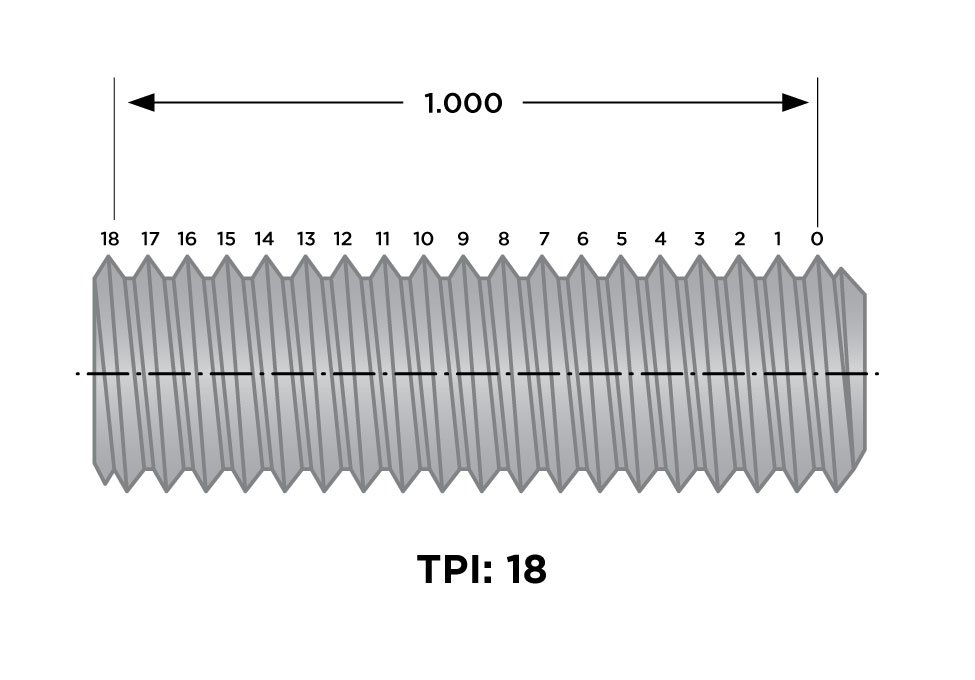
\includegraphics{Introduction to Nut and Bolt Sizes_files/62ffe00403d64741542980.jpg}
		
		\hypertarget{i5uow1}{}
		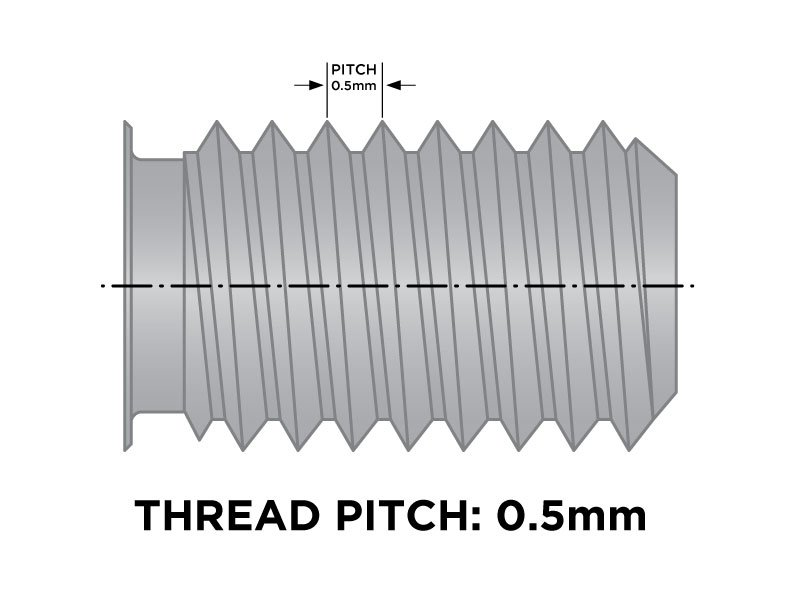
\includegraphics{Introduction to Nut and Bolt Sizes_files/62ffe01b5939b908779409.jpg}
		
		\hypertarget{iazchh}{%
			\subsubsection{Measurement Format for Size Names}\label{iazchh}}
		
		\hypertarget{ialm3q}{}
		Nut and bolt size names, regardless of the measurement system, are
		always given as the \textbf{OD followed by the TPI or thread pitch} .
		The names within each measurement system will look slightly different.
		
		\hypertarget{iof4zr}{%
			\paragraph{Inch Format}\label{iof4zr}}
		
		\hypertarget{ihinup}{}
		The measurement of an inch nut or bolt will be listed as the
		\emph{thread size} --- a number between one and 12 or an inch increment
		followed by the threads per inch (TPI). If the diameter is less than 1/4
		inch, the diameter will be listed as a number between zero and 12; the
		larger the number, the closer it is to 1/4 inch. When the diameter is
		equal to or larger than 1/4 inch, it will be listed as an inch
		increment.
		
		\begin{longtable}[]{@{}ll@{}}
			\toprule
			\begin{minipage}[b]{0.47\columnwidth}\raggedright
				\hypertarget{ip8vlo}{}
				Thread Size\strut
			\end{minipage} & \begin{minipage}[b]{0.47\columnwidth}\raggedright
				\hypertarget{ilg6c1}{}
				OD\strut
			\end{minipage}\tabularnewline
			\midrule
			\endhead
			\begin{minipage}[t]{0.47\columnwidth}\raggedright
				\hypertarget{ij13wo}{}
				\#10 - 32\strut
			\end{minipage} & \begin{minipage}[t]{0.47\columnwidth}\raggedright
				\hypertarget{imhx99}{}
				0.19"\strut
			\end{minipage}\tabularnewline
			\begin{minipage}[t]{0.47\columnwidth}\raggedright
				\hypertarget{iofufv}{}
				\#12 - 24\strut
			\end{minipage} & \begin{minipage}[t]{0.47\columnwidth}\raggedright
				\hypertarget{i5dvs2}{}
				0.216"\strut
			\end{minipage}\tabularnewline
			\begin{minipage}[t]{0.47\columnwidth}\raggedright
				\hypertarget{iwitbx}{}
				1/4" - 20\strut
			\end{minipage} & \begin{minipage}[t]{0.47\columnwidth}\raggedright
				\hypertarget{i2rpr7}{}
				0.25"\strut
			\end{minipage}\tabularnewline
			\begin{minipage}[t]{0.47\columnwidth}\raggedright
				\hypertarget{icppsh}{}
				5/16" - 18\strut
			\end{minipage} & \begin{minipage}[t]{0.47\columnwidth}\raggedright
				\hypertarget{ie9zwk}{}
				0.3125"\strut
			\end{minipage}\tabularnewline
			\bottomrule
		\end{longtable}
		
		\hypertarget{ii5xkl}{}
		The TPI, or number of threads within an inch of the thread length, will
		immediately follow the diameter.
		
		\hypertarget{iujivc}{}
		\textbf{Example 1:} \#6-24 (\#6 = 0.138 in. OD; 24 = 24 threads in one
		inch of thread length)
		
		\textbf{Example 2:} 1/4"-28 (1/4 = 1/4 in. OD; 28 = 28 threads in one
		inch of thread length)
		
		\hypertarget{i7byi7f}{%
			\paragraph{Metric Format}\label{i7byi7f}}
		
		\hypertarget{ibz5no}{}
		The thread size of a metric nut or bolt is listed as the letter "M"
		followed by a number that indicates the number of millimeters across the
		diameter and then the thread pitch.
		
		\hypertarget{ivmq62}{}
		\textbf{Example:} M4 x 0.7 (M4 = 4 mm OD; 0.7 = 0.7 mm between thread
		crests)
		
		\hypertarget{ia6doav}{%
			\subsubsection{Coarse and Fine Threads}\label{ia6doav}}
		
		\hypertarget{i5h0xk}{}
		Nut and bolt size names will sometimes also factor in whether the thread
		is coarse or fine. Simply put, coarse threads are thicker and farther
		apart from each other, while fine threads are thinner and closer
		together.
		
		\hypertarget{i56kg7}{}
		There are a few acronymns that are used to designate each thread type:
		
		\hypertarget{im72dg}{%
			\paragraph{Standard Coarse Threads}\label{im72dg}}
		
		\begin{itemize}
			\tightlist
			\item
			\textbf{UNC:} Unified National Coarse threads comparable to ISO metric
			threads
			\item
			\textbf{UNRC:} Unified National Coarse threads; the "R" indicates
			"rolled" external threads that have a rounded root contour. They are
			full interchangeable with UNC fasteners.
			\item
			\textbf{UNJC:} Unified National Coarse threads with an increased minor
			diameter and controlled root radius that disperses tensile strength
			over a broader area. Derived from a military specification
			(MIL-S-8879), they are designed for high stress applications. However,
			they are not interchangeable with other UNC fasteners.
		\end{itemize}
		
		\hypertarget{iyqv5s}{%
			\paragraph{Metric Coarse Threads}\label{iyqv5s}}
		
		\begin{itemize}
			\tightlist
			\item
			ISO metric threads will simply use the word \textbf{"coarse."}
		\end{itemize}
		
		\hypertarget{ixrtlg}{%
			\paragraph{Standard Fine Threads}\label{ixrtlg}}
		
		\begin{itemize}
			\tightlist
			\item
			\textbf{UNF:} Unified National Fine threads.
			\item
			\textbf{UNRF:} Unified National Fine threads; the "R" indicates
			"rolled" external threads that have a rounded root contour. They are
			fully interchangeable with other UNF fasteners.
			\item
			\textbf{UNJF:} Unified National Fine threads with an increased minor
			diameter and controlled root radius that disperses tensile stress over
			a broader area. Derived from a military specification (MIL-S-8879),
			they are designed for high stress applications. However, they are not
			interchangeable with other UNF fasteners.
		\end{itemize}
		
		\hypertarget{ipqpdr}{%
			\paragraph{Metric Fine Threads}\label{ipqpdr}}
		
		\begin{itemize}
			\tightlist
			\item
			ISO metric threads will simply use the words~\textbf{"fine"}{~or
				\textbf{"super fine."}}
		\end{itemize}
		
		\hypertarget{ie6q5l}{}
		Sometimes, you will see the same thread size listed twice, each with a
		different thread pitch or TPI next to them. For example:
		
		\begin{itemize}
			\tightlist
			\item
			\textbf{M2.3 x 0.45 vs. M2.3 x 0.4:} These have the same diameter, but
			the thread pitch in the first measurement is larger than the second
			one, so the distance between threads will be bigger.
			\item
			\textbf{\#10 - 24 vs. \#10 - 32:} These have the same diameter, but
			the TPI in the first measurement is lower than the second one, so
			there will be fewer threads per inch of thread length.
		\end{itemize}
		
		\hypertarget{iivm5l}{}
		Because TPIs and thread pitches are calculated differently, remember the
		following:
		
		\begin{itemize}
			\tightlist
			\item
			\textbf{Inch Threads:} A higher TPI indicates finer threads as there
			are more threads within an inch of thread length.
			\item
			\textbf{Metric Threads:} A lower thread pitch indicates finer threads
			as there is less space between each thread crest.
		\end{itemize}
		
		\hypertarget{ibnyqd}{%
			\subsection{Standards}\label{ibnyqd}}
		
		\hypertarget{icngzy}{}
		Nuts and bolts are regulated by
		\href{https://www.huyett.com/blog-why-are-standards-important}{standards},
		depending on their measurement system.
		
		\hypertarget{iibhbc}{%
			\subsubsection{Inch Standards}\label{iibhbc}}
		
		\hypertarget{i9sheb}{}
		As our \href{https://www.huyett.com/blog-nuts-and-bolts}{Guide to Nuts
			and Bolts} explains, most inch nuts and bolts comply with the Unified
		Thread Standard (UTS). The American Society of Mechanical Engineers
		(ASME) and The American National Standards Institute (ANSI) regulate
		this standard. Additionally, the Society of Automotive Engineers (SAE
		International) regulates standards for parts used in automotive
		applications. If any of the following standards apply to your nuts or
		bolts, you are working with inch fasteners:
		
		\begin{itemize}
			\tightlist
			\item
			\textbf{UTS:} Unified Thread Standard for screw threads commonly used
			in the U.S. and Canada including Unified National Coarse (UNC) and
			Unified National Fine (UNF) threads. ASME/ANSI --- Specifies screw
			thread properties for three classes of general purpose unified screw
			threads including: UN, UNR, and UNJ series fasteners.
			\item
			\textbf{SAE:} A standard that designates the number of threads per
			inch for coarse and fine American (or standard) bolts, screws, pipes,
			ports, and flange ports.
		\end{itemize}
		
		\hypertarget{i9a69k}{%
			\subsubsection{Metric Standards}\label{i9a69k}}
		
		\hypertarget{iqka0h}{}
		For metric nuts and bolts, the most common standards are:
		
		\begin{itemize}
			\tightlist
			\item
			\textbf{ISO:} Strict specifications for coarse, fine, and superfine
			metric threads defined by the International Organization for
			Standardization.
			\item
			\textbf{DIN:} Standards defined by the German Institute for
			Standardization (or Deutsches Institut für Normung, hence "DIN") for
			thread styles commonly used in Europe.
		\end{itemize}
		
		\hypertarget{iqn22v}{%
			\subsubsection{ASTM}\label{iqn22v}}
		
		\hypertarget{i8rga1s}{}
		The American Society for Testing and Materials (ASTM) standard covers
		both inch and metric nuts and bolts. We'll discuss how to identify the
		appropriate measurement system in the following section.
		
		\hypertarget{iaa4t5o}{%
			\subsection{Strength Grade Markings}\label{iaa4t5o}}
		
		\hypertarget{i0htiud}{}
		Sometimes, manufacturers mark their nuts and bolts with indentations to
		indicate the strength of the fastener. Different standards use different
		strength markings, but there are a few markings you are most likely to
		encounter.
		
		\hypertarget{iw5uma}{%
			\subsubsection{Inch Grade Markings}\label{iw5uma}}
		
		\hypertarget{i7qq3fl}{}
		Inch nuts regulated by the SAE will have lengthwise lines within the
		circle on the top of the nut, while bolts will have lines on the bolt
		head moving from the center of the head outwards.
		
		\hypertarget{in8paa}{}
		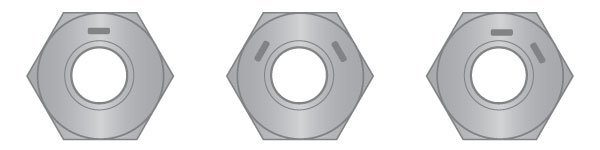
\includegraphics{Introduction to Nut and Bolt Sizes_files/6307b8d27e9fd904635918.jpg}
		
		\hypertarget{ivmctl}{}
		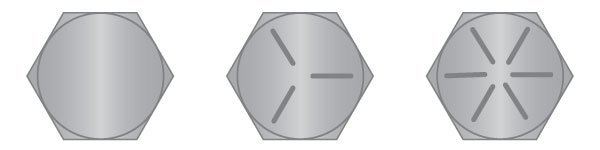
\includegraphics{Introduction to Nut and Bolt Sizes_files/6307b8fa19b82843920771.jpg}
		
		\hypertarget{i7ab7i}{%
			\subsubsection{Metric Grade Markings}\label{i7ab7i}}
		
		\hypertarget{i3f3hj}{}
		If a nut or bolt shows numbers instead of line indentations to indicate
		their strength grade, it is a metric fastener. However, depending on the
		fastener's standard, metric nuts can also show a pattern of lines and
		dots between the circle and the sides of the nuts. Metric nuts will
		print these indentations outside the circle.
		
		\hypertarget{i6g3ac}{}
		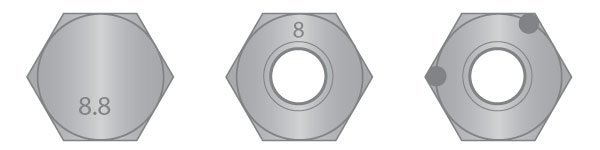
\includegraphics{Introduction to Nut and Bolt Sizes_files/6307b947273e3119595489.jpg}
		
		\hypertarget{iawz2f}{}
		
		\hypertarget{in2ujb}{%
			\subsubsection{ASTM Grade Markings}\label{in2ujb}}
		
		\hypertarget{ibwq7f}{}
		You may also come across bolts with alphanumeric marks, typically an
		"A," "B," or "F" in combination with one to four numbers. This mark
		could exist on its own or along with lines. This is an ASTM strength
		grade mark. If this mark is followed by a capital "M," that signifies
		that the fastener is metric. If there is no "M" present, it is an inch
		fastener.
		
		\hypertarget{ioka1w}{}
		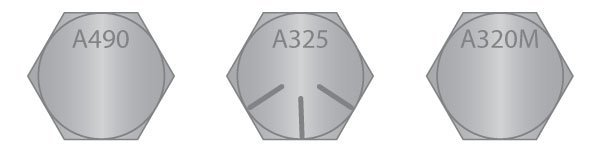
\includegraphics{Introduction to Nut and Bolt Sizes_files/6307b985e0134715291439.jpg}
		
		\hypertarget{i2x1zy}{}
		
		\hypertarget{ite14y}{}
		Manufacturers are not required to mark their fasteners with strength
		grades, so this is not a guaranteed method of identifying the inch or
		metric designation of your fastener. Many nuts and bolts will only
		imprint the manufacturer's brand mark, which may be a simple letter and
		should not be confused with a strength grade.
		
		\hypertarget{i72lz7}{%
			\subsection{How to Identify Your Nut and Bolt
				Measurements}\label{i72lz7}}
		
		\hypertarget{iw4hn7}{}
		There are times you will need to identify the measurements of your nuts
		and bolts from scratch. There is no exact way to do this without
		specific tools, but you can narrow down the key measurements with a
		basic inch and metric ruler. From here, you can take your fasteners to a
		local hardware store and locate the closest match.
		
		\hypertarget{ilxb3s}{}
		To identify the nut and bolt measurements:
		
		\begin{itemize}
			\tightlist
			\item
			First, determine if you are working with inch or standard fasteners by
			identifying the standard associated with your nut or bolt or by
			looking at the bolt head or the top of the screw. If there are visible
			markings, refer to the previous descriptions.
			\item
			If you are unable to determine the measurement system, you'll need to
			record the OD in both inches and millimeters.
		\end{itemize}
		
		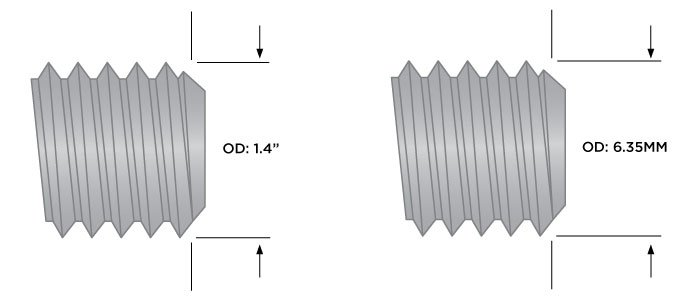
\includegraphics{Introduction to Nut and Bolt Sizes_files/6307ba3bb06ad783039359.jpg}
		
		\begin{itemize}
			\tightlist
			\item
			OD in Inches and Millimeters
			\item
			Measure an inch of the thread length and count the number of threads
			within the inch to determine the TPI.
			\item
			Measure the distance between threads in millimeters to determine the
			thread pitch.
			\item
			Using the OD measured in inches and the TPI, assemble the standard
			version of your measurement. It should look like: \textbf{inch
				OD-TPI}. (Example: 1/4"-28)
			\item
			Using the OD measured in millimeters and the thread pitch, assemble
			the metric version of your measurement. It should look like: \textbf{M
				OD x thread pitch}. (Example: M4 x 0.7)
			\item
			Take both versions of these measurements to a local hardware store;
			you can then identify the fasteners with the closest measurements to
			yours.
			\item
			For more accurate measurements, consider investing in inch and metric
			thread gauges. These small tools look like pocket knives and hold fans
			of blades with different sized notches. The notches correspond to
			thread sizes, which are marked on the blade. Press the threads of your
			part against the different blades until you find the blade that
			nestles perfectly on the threads. This will not only tell you whether
			your part is an inch or metric part, but it will also narrow down the
			exact TPI or thread pitch.
			\item
			Remember not to mix standard and metric fasteners. They are designed
			to work with appropriately-mating parts; if you mix a standard bolt
			with a metric nut, the threads may not hold correctly. This can cause
			damage to your application and could be a safety concern.
		\end{itemize}
		
		\hypertarget{iz6h0v3}{%
			\subsection{Measurement Charts}\label{iz6h0v3}}
		
		\hypertarget{idtx4l}{}
		Size charts for nuts and bolts can cover a variety of measurements. Ours
		cover common nut and bolt sizes for fasteners with ODs up to 1" and
		25mm. We include the following essential measurements:
		
		\begin{itemize}
			\tightlist
			\item
			\textbf{Thread size:} This indicates the full size name. For inch
			fasteners, this is the OD followed by the TPI. For metric fasteners,
			an "M" is followed by the OD, which is then followed by the thread
			pitch.
			\item
			\textbf{Outside diameter (OD):} This is the basic actual measurement
			that correlates with the thread size.
			\item
			\textbf{TPI/Thread Pitch:} The standard chart lists the correlating
			TPI, while the metric chart lists the correlating thread pitch.
			\item
			\textbf{Coarse/Fine Thread Designation:} The standard chart uses the
			"UN" acronymns explained above, while the metric chart uses the words
			"coarse" and "fine" in accordance with ISO's designations.
		\end{itemize}
		
		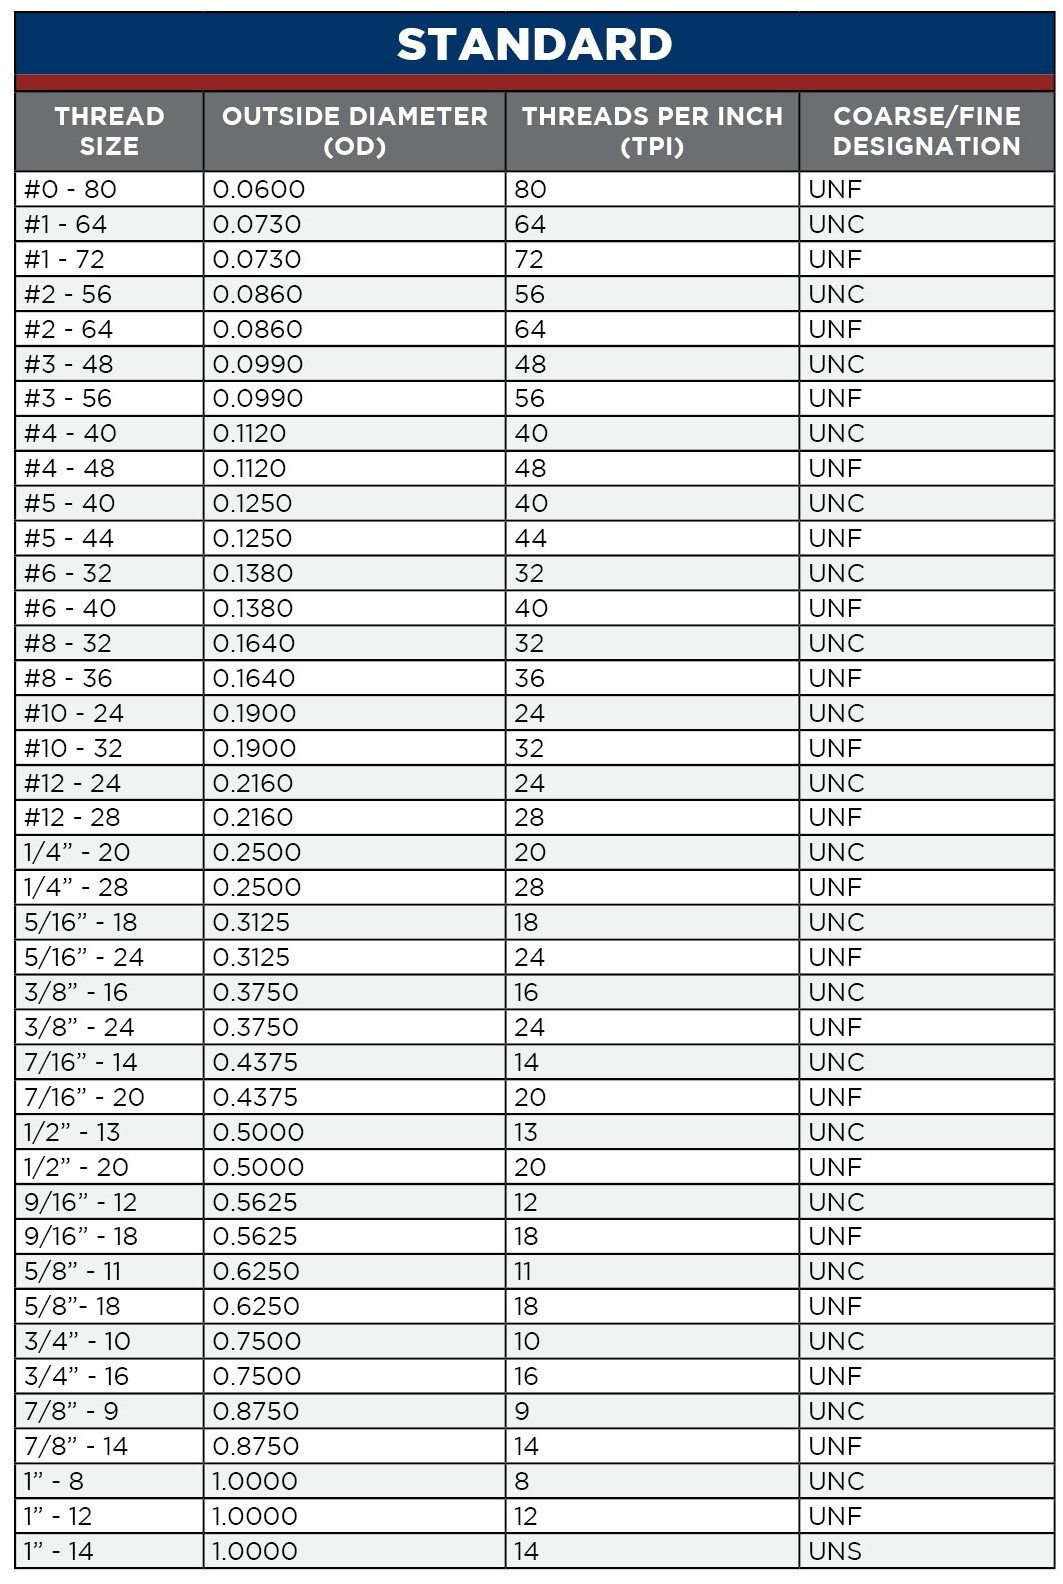
\includegraphics{Introduction to Nut and Bolt Sizes_files/6307bab88eccb893095369.jpg}
		\newpage
		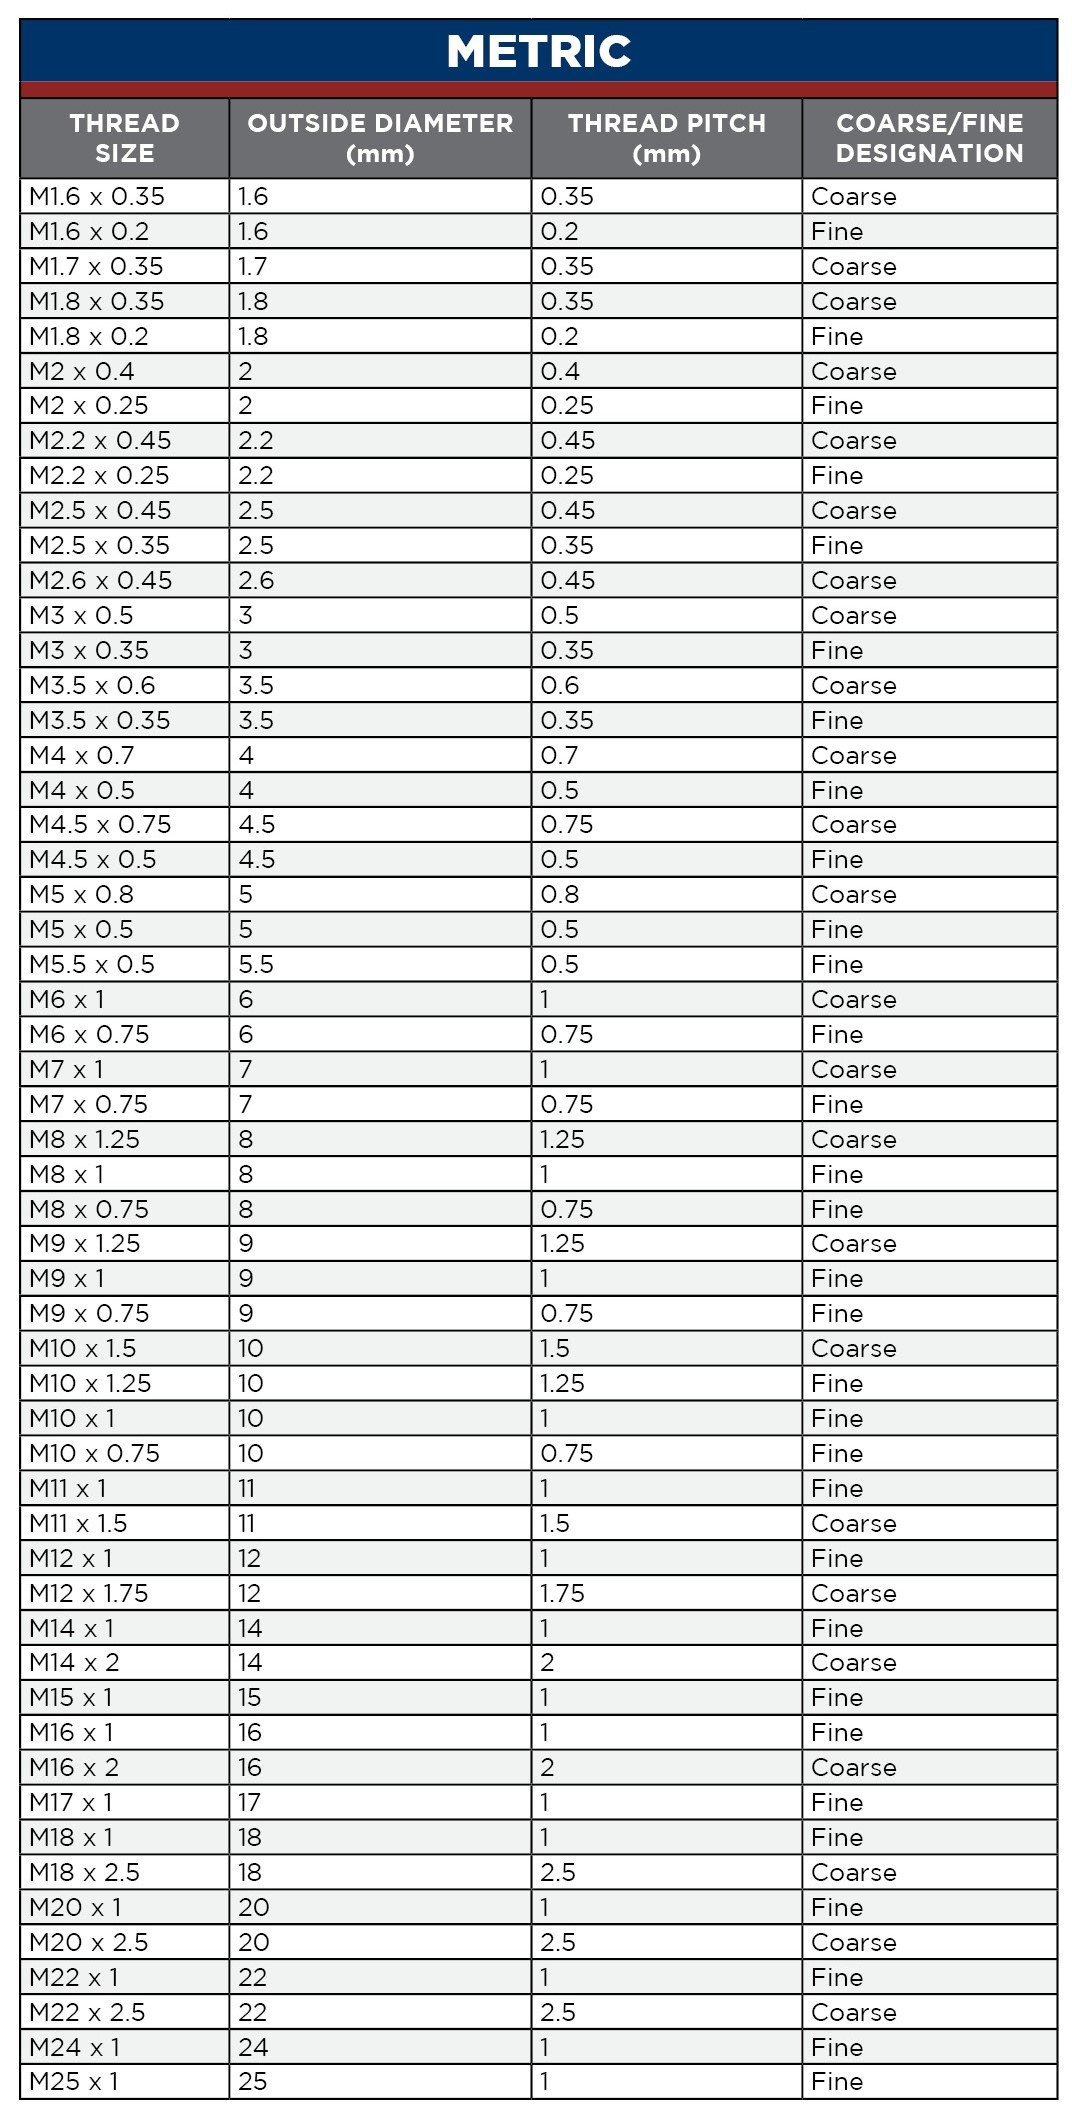
\includegraphics{Introduction to Nut and Bolt Sizes_files/6307baf81ff28690984895.jpg}
		
		\hypertarget{iqru7da}{%
			\subsection{Other Measurements for Common Nut and Bolt
				Types}\label{iqru7da}}
		
		\hypertarget{i7aa4wx}{}
		While the outside diameter and TPI/thread pitch are the essential
		measurements for every type of nut or bolt, different types of fasteners
		have other unique measurements that are important to know.
		
		\hypertarget{ifa94lv}{%
			\subsubsection{Nuts}\label{ifa94lv}}
		
		\hypertarget{if13qfk}{}
		Most \href{https://www.huyett.com/all-products/nuts}{nuts} have three
		main measurements beyond the OD and TPI/thread pitch:
		
		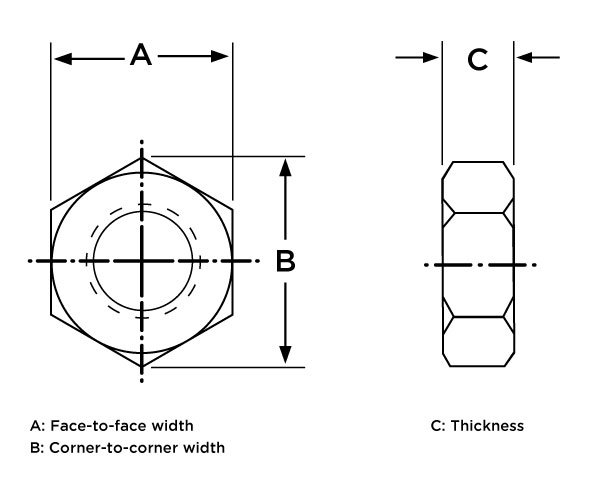
\includegraphics{Introduction to Nut and Bolt Sizes_files/6307bb72dbb49891453363.jpg}
		
		\hypertarget{ijs7afj}{}
		A: Face-to-face width; B: Corner-to-corner width; C: Thickness
		
		\hypertarget{isfuo09}{}
		Exceptions to this are
		\href{https://www.huyett.com/all-products/nuts/wing-nuts}{wing nuts},
		which are decidedly different shapes than nuts with hex shapes like
		\href{https://www.huyett.com/all-products/nuts/hex-nuts}{hex nuts},
		\href{https://www.huyett.com/all-products/nuts/coupling-nuts}{coupling
			nuts}, \href{https://www.huyett.com/all-products/nuts/lock-nuts}{lock
			nuts}, and
		\href{https://www.huyett.com/all-products/nuts/lock-nuts/jam-lock-nuts}{jam
			nuts}.
		
		\hypertarget{ipyz34t}{%
			\paragraph{Wing Nut}\label{ipyz34t}}
		
		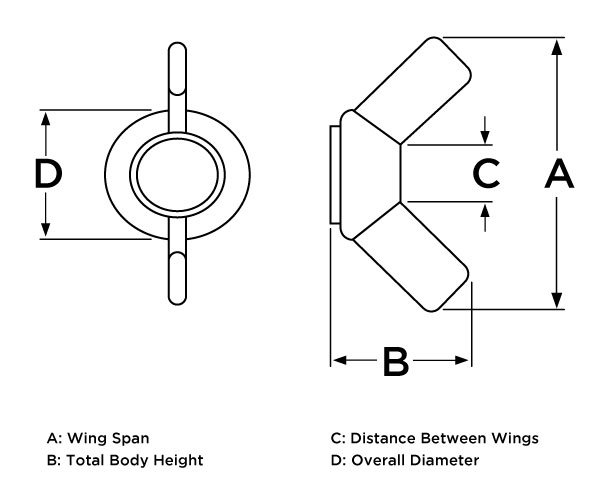
\includegraphics{Introduction to Nut and Bolt Sizes_files/6307bc42ebae7262807955.jpg}
		
		\hypertarget{ira03ji}{}
		A: Wing Span; B: Total Body Height; C: Distance Between Wings; D:
		Overall Diameter
		
		\hypertarget{iruib3g}{%
			\subsubsection{Bolts}\label{iruib3g}}
		
		\hypertarget{i921nmg}{}
		There are a wide variety of bolt types with unique features and profiles
		that require unique measurement callouts.
		
		\hypertarget{i45vs4o}{}
		\hypertarget{iygv1bu}{}
		\hypertarget{ikau5po}{%
			\paragraph{\texorpdfstring{\href{https://www.huyett.com/all-products/bolts/hex-bolts}{Hex
						Bolts}}{Hex Bolts}}\label{ikau5po}}
		
		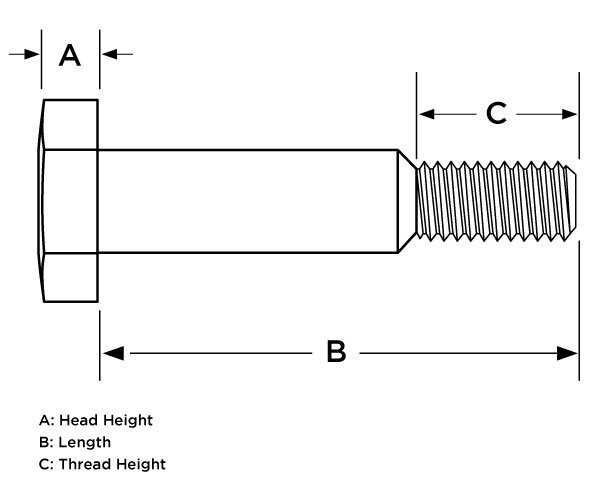
\includegraphics{Introduction to Nut and Bolt Sizes_files/6307bd0a95270402904591.jpg}
		
		\hypertarget{izm4mmm}{}
		A: Head Height; B: Length; C: Thread Height
		
		\hypertarget{igkw95g}{}
		\hypertarget{i5213mh}{%
			\paragraph{\texorpdfstring{\href{https://www.huyett.com/all-products/bolts/eye-bolts}{Lifting
						Eye Bolts}}{Lifting Eye Bolts}}\label{i5213mh}}
		
		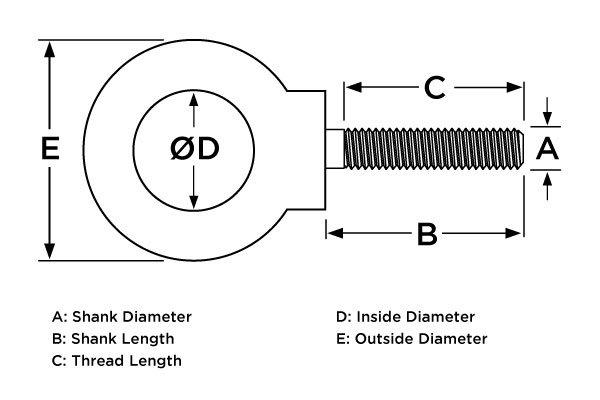
\includegraphics{Introduction to Nut and Bolt Sizes_files/6307bcfa5c57d694202170.jpg}
		
		\hypertarget{ijtjve5}{}
		A: Shank Diameter; B: Shank Length; C: Thread Length; D: Inside
		Diameter; E: Outside Diameter
		
		\hypertarget{i9gqtac}{}
		\hypertarget{i8b9v29}{}
		\hypertarget{il3jc1y}{%
			\paragraph{\texorpdfstring{\href{https://www.huyett.com/product/search?search=l-bolt}{L-Bolts}}{L-Bolts}}\label{il3jc1y}}
		
		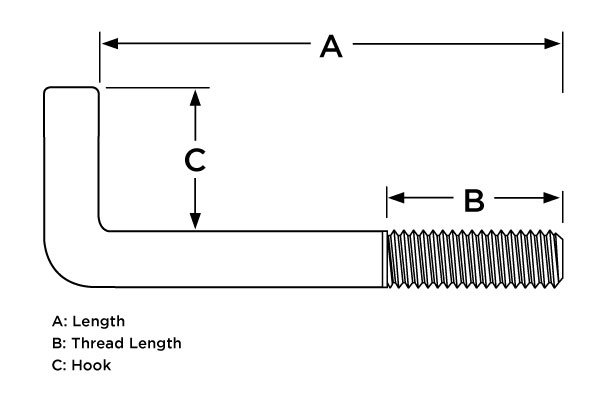
\includegraphics{Introduction to Nut and Bolt Sizes_files/6307bd9dd0447291869107.jpg}
		
		\hypertarget{i9y9v8n}{}
		A: Length; B: Thread Length; C: Hook
		
		\hypertarget{iob5e0i}{}
		\hypertarget{in9zoqf}{%
			\paragraph{\texorpdfstring{\href{https://www.huyett.com/all-products/bolts/u-bolts}{U-Bolts}}{U-Bolts}}\label{in9zoqf}}
		
		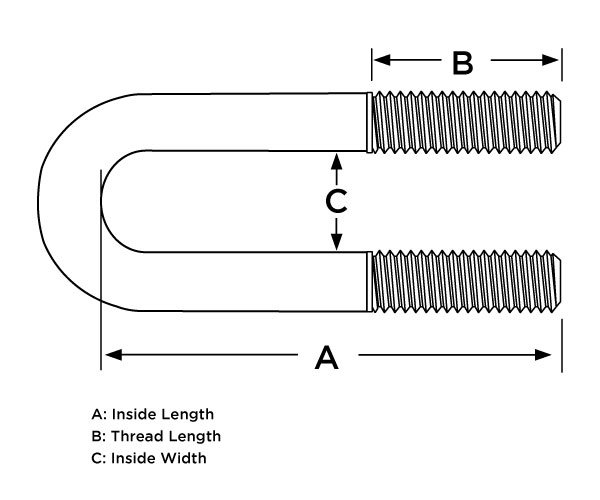
\includegraphics{Introduction to Nut and Bolt Sizes_files/6307bd701bf44407484420.jpg}
		
		\hypertarget{iceu7t3}{}
		A: Inside Length; B: Thread Length; C: Inside Width
		
		\hypertarget{i6ize6}{}
		\hypertarget{ilxlvm}{%
			\paragraph{\texorpdfstring{\href{https://www.huyett.com/product/search?search=step\%20bolt}{Step
						Bolts}}{Step Bolts}}\label{ilxlvm}}
		
		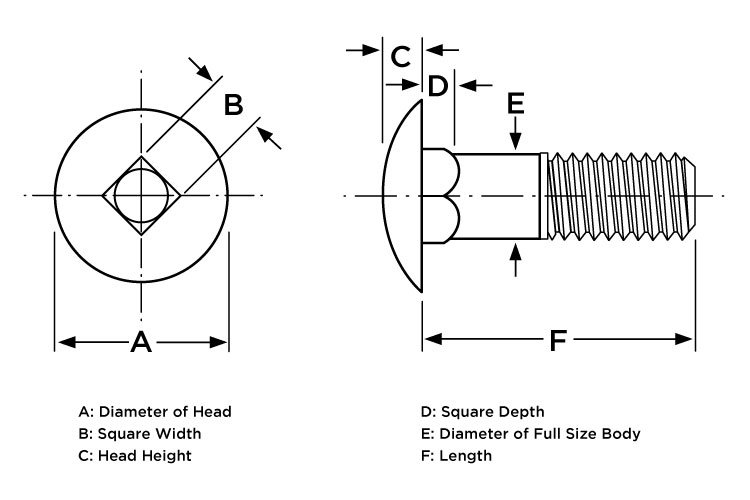
\includegraphics{Introduction to Nut and Bolt Sizes_files/6307c769a225a243287054.jpg}
		
		\hypertarget{iba6cl}{}
		A: Diameter of Head; B: Square Width; C: Head Height; D: Square Depth;
		E: Diameter of Full Size Body; F: Length
		
		\hypertarget{irkmnp}{}
	
\end{document}